\documentclass[11pt]{article}
\usepackage[margin=1in]{geometry}
\usepackage{booktabs}
\usepackage{graphicx}
\usepackage{longtable}
\usepackage{hyperref}
\title{Kazakhstan Unemployment Forecasting Report}
\author{[Author Name]}
\date{\today}
\begin{document}
\maketitle

\section{Objective}
[Describe research question, policy relevance, and forecasting horizon.]

\section{Data and Preprocessing}
[Describe data sources, transformations, merge logic, and date handling.]

\section{Methodology}
\subsection{Feature Engineering}
[Describe Fourier terms, lags, rolling statistics (shifted to avoid lookahead),
interactions, dummies, structural breaks, PCA.]

\subsection{Model Stack}
[Describe SARIMAX (stationarity enforced), VARX, ElasticNet,
XGBoost (trained on differenced target), and Prophet.]

\subsection{Validation Protocol}
[Describe 24-month recursive walk-forward evaluation from 2024-01 to 2025-12.
Recursive means predicted values substitute actual lags for multi-step horizons.]

\section{Results}
\begin{table}
\caption{Out-of-sample performance (walk-forward, 2024-01 to 2025-12).}
\label{tab:model_metrics}
\begin{tabular}{lrrr}
\toprule
Model & MAE & RMSE & R2 \\
\midrule
ElasticNet & 0.0062 & 0.0204 & 0.7773 \\
Ensemble & 0.0063 & 0.0203 & 0.7810 \\
XGBoost & 0.0067 & 0.0202 & 0.7833 \\
SARIMAX & 0.0262 & 0.0342 & 0.3749 \\
VARX & 0.0300 & 0.0413 & 0.0887 \\
Prophet & 0.0317 & 0.0389 & 0.1912 \\
SeasonalNaive & 0.0625 & 0.0791 & -2.3333 \\
\bottomrule
\end{tabular}
\end{table}


\section{Diagnostics}
\begin{figure}[h!]
    \centering
    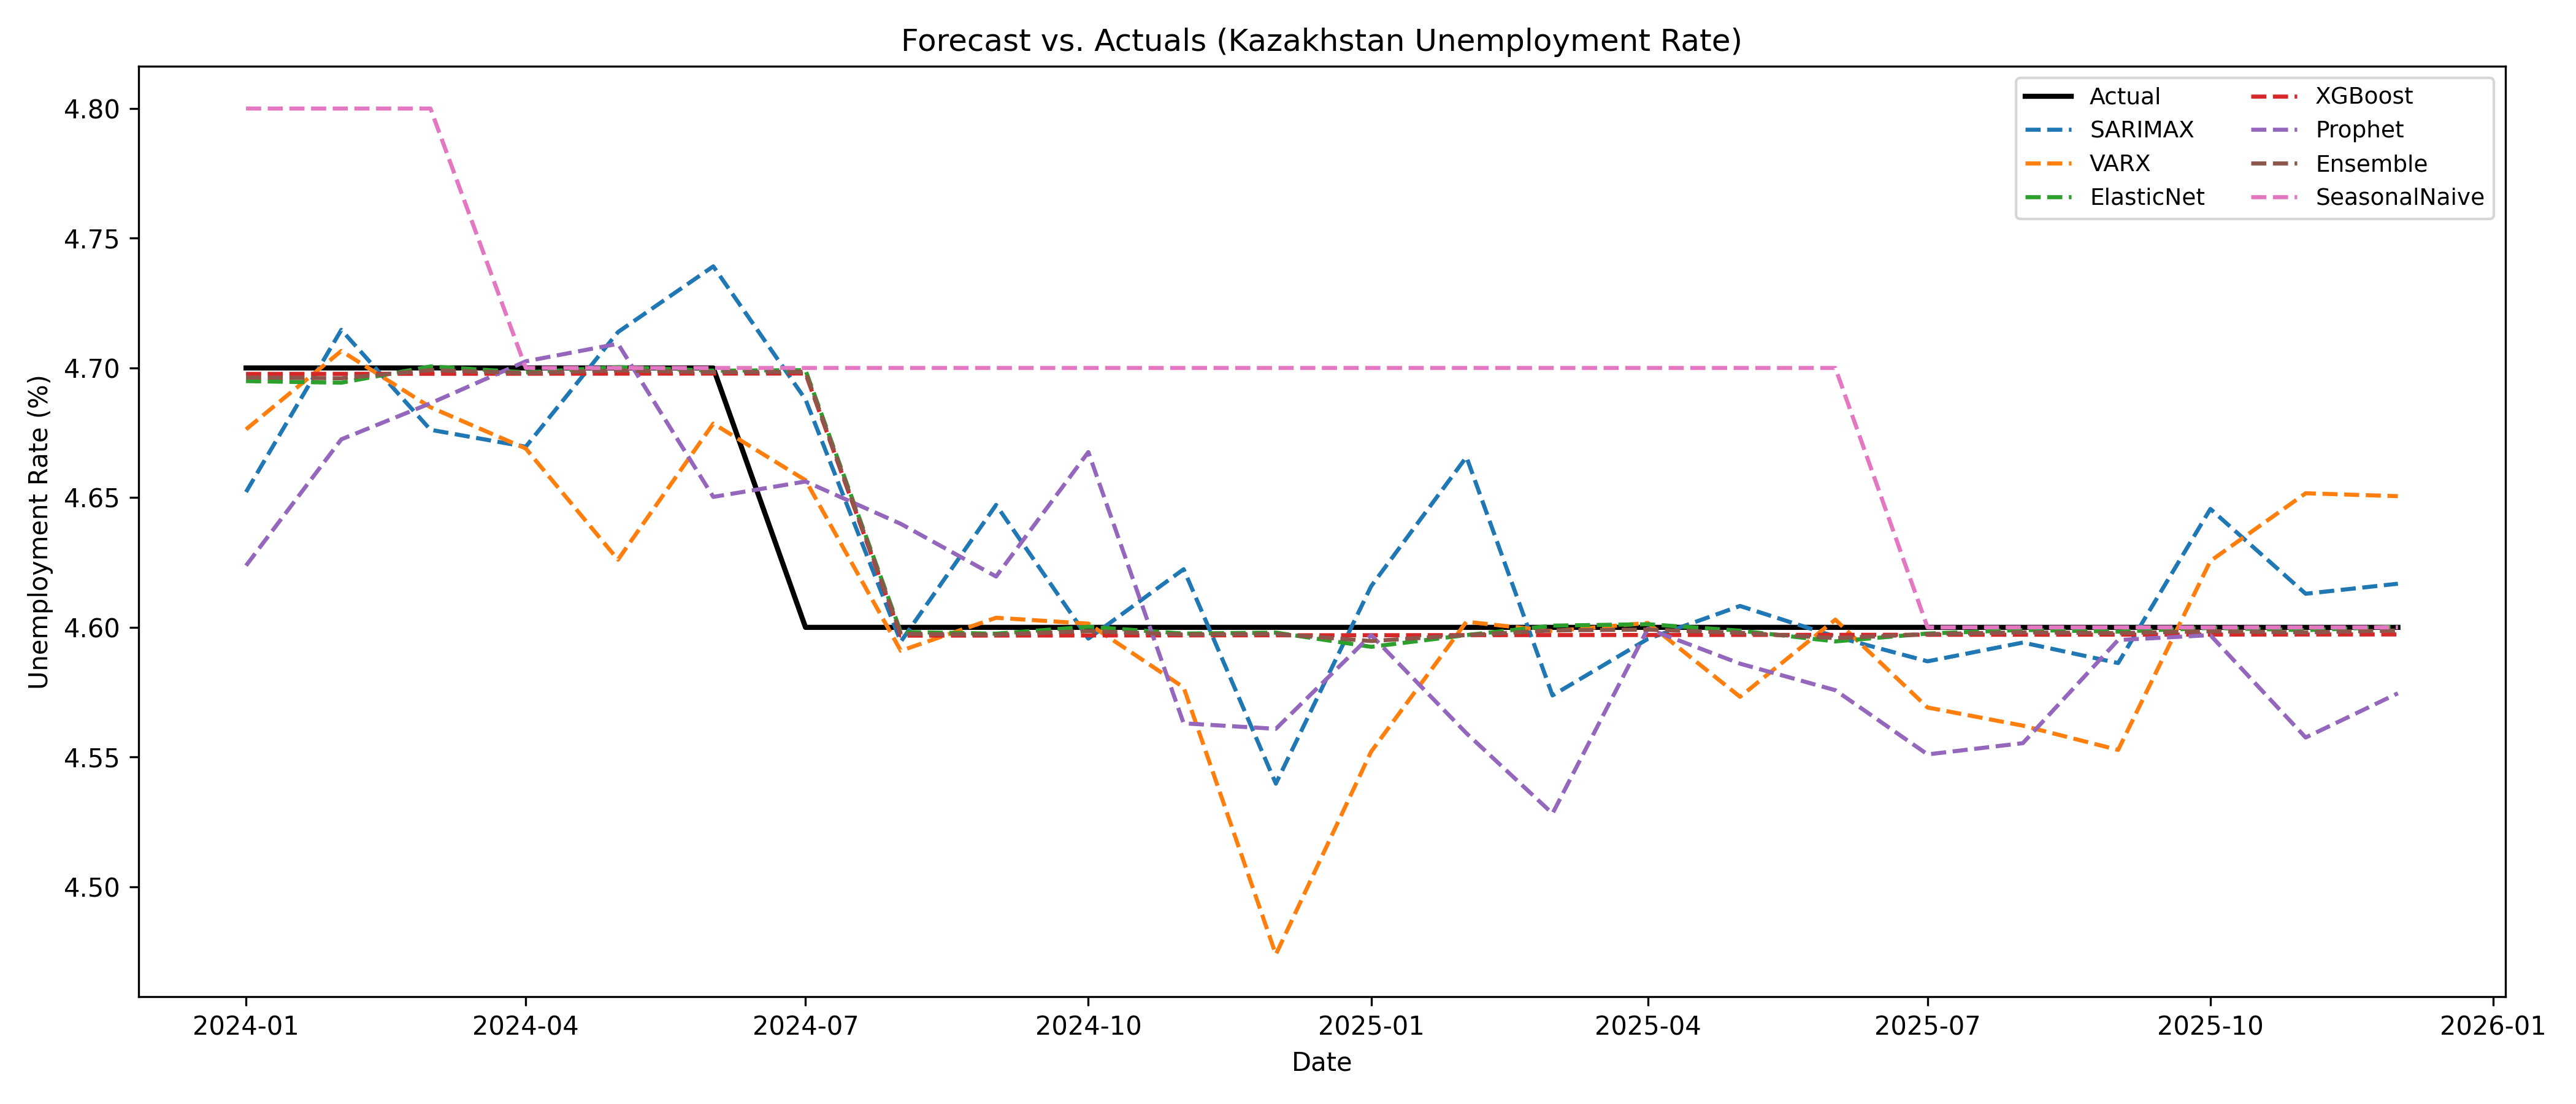
\includegraphics[width=0.9\textwidth]{figures/forecast_vs_actuals.png}
    \caption{Forecast vs. Actuals}
\end{figure}

\begin{figure}[h!]
    \centering
    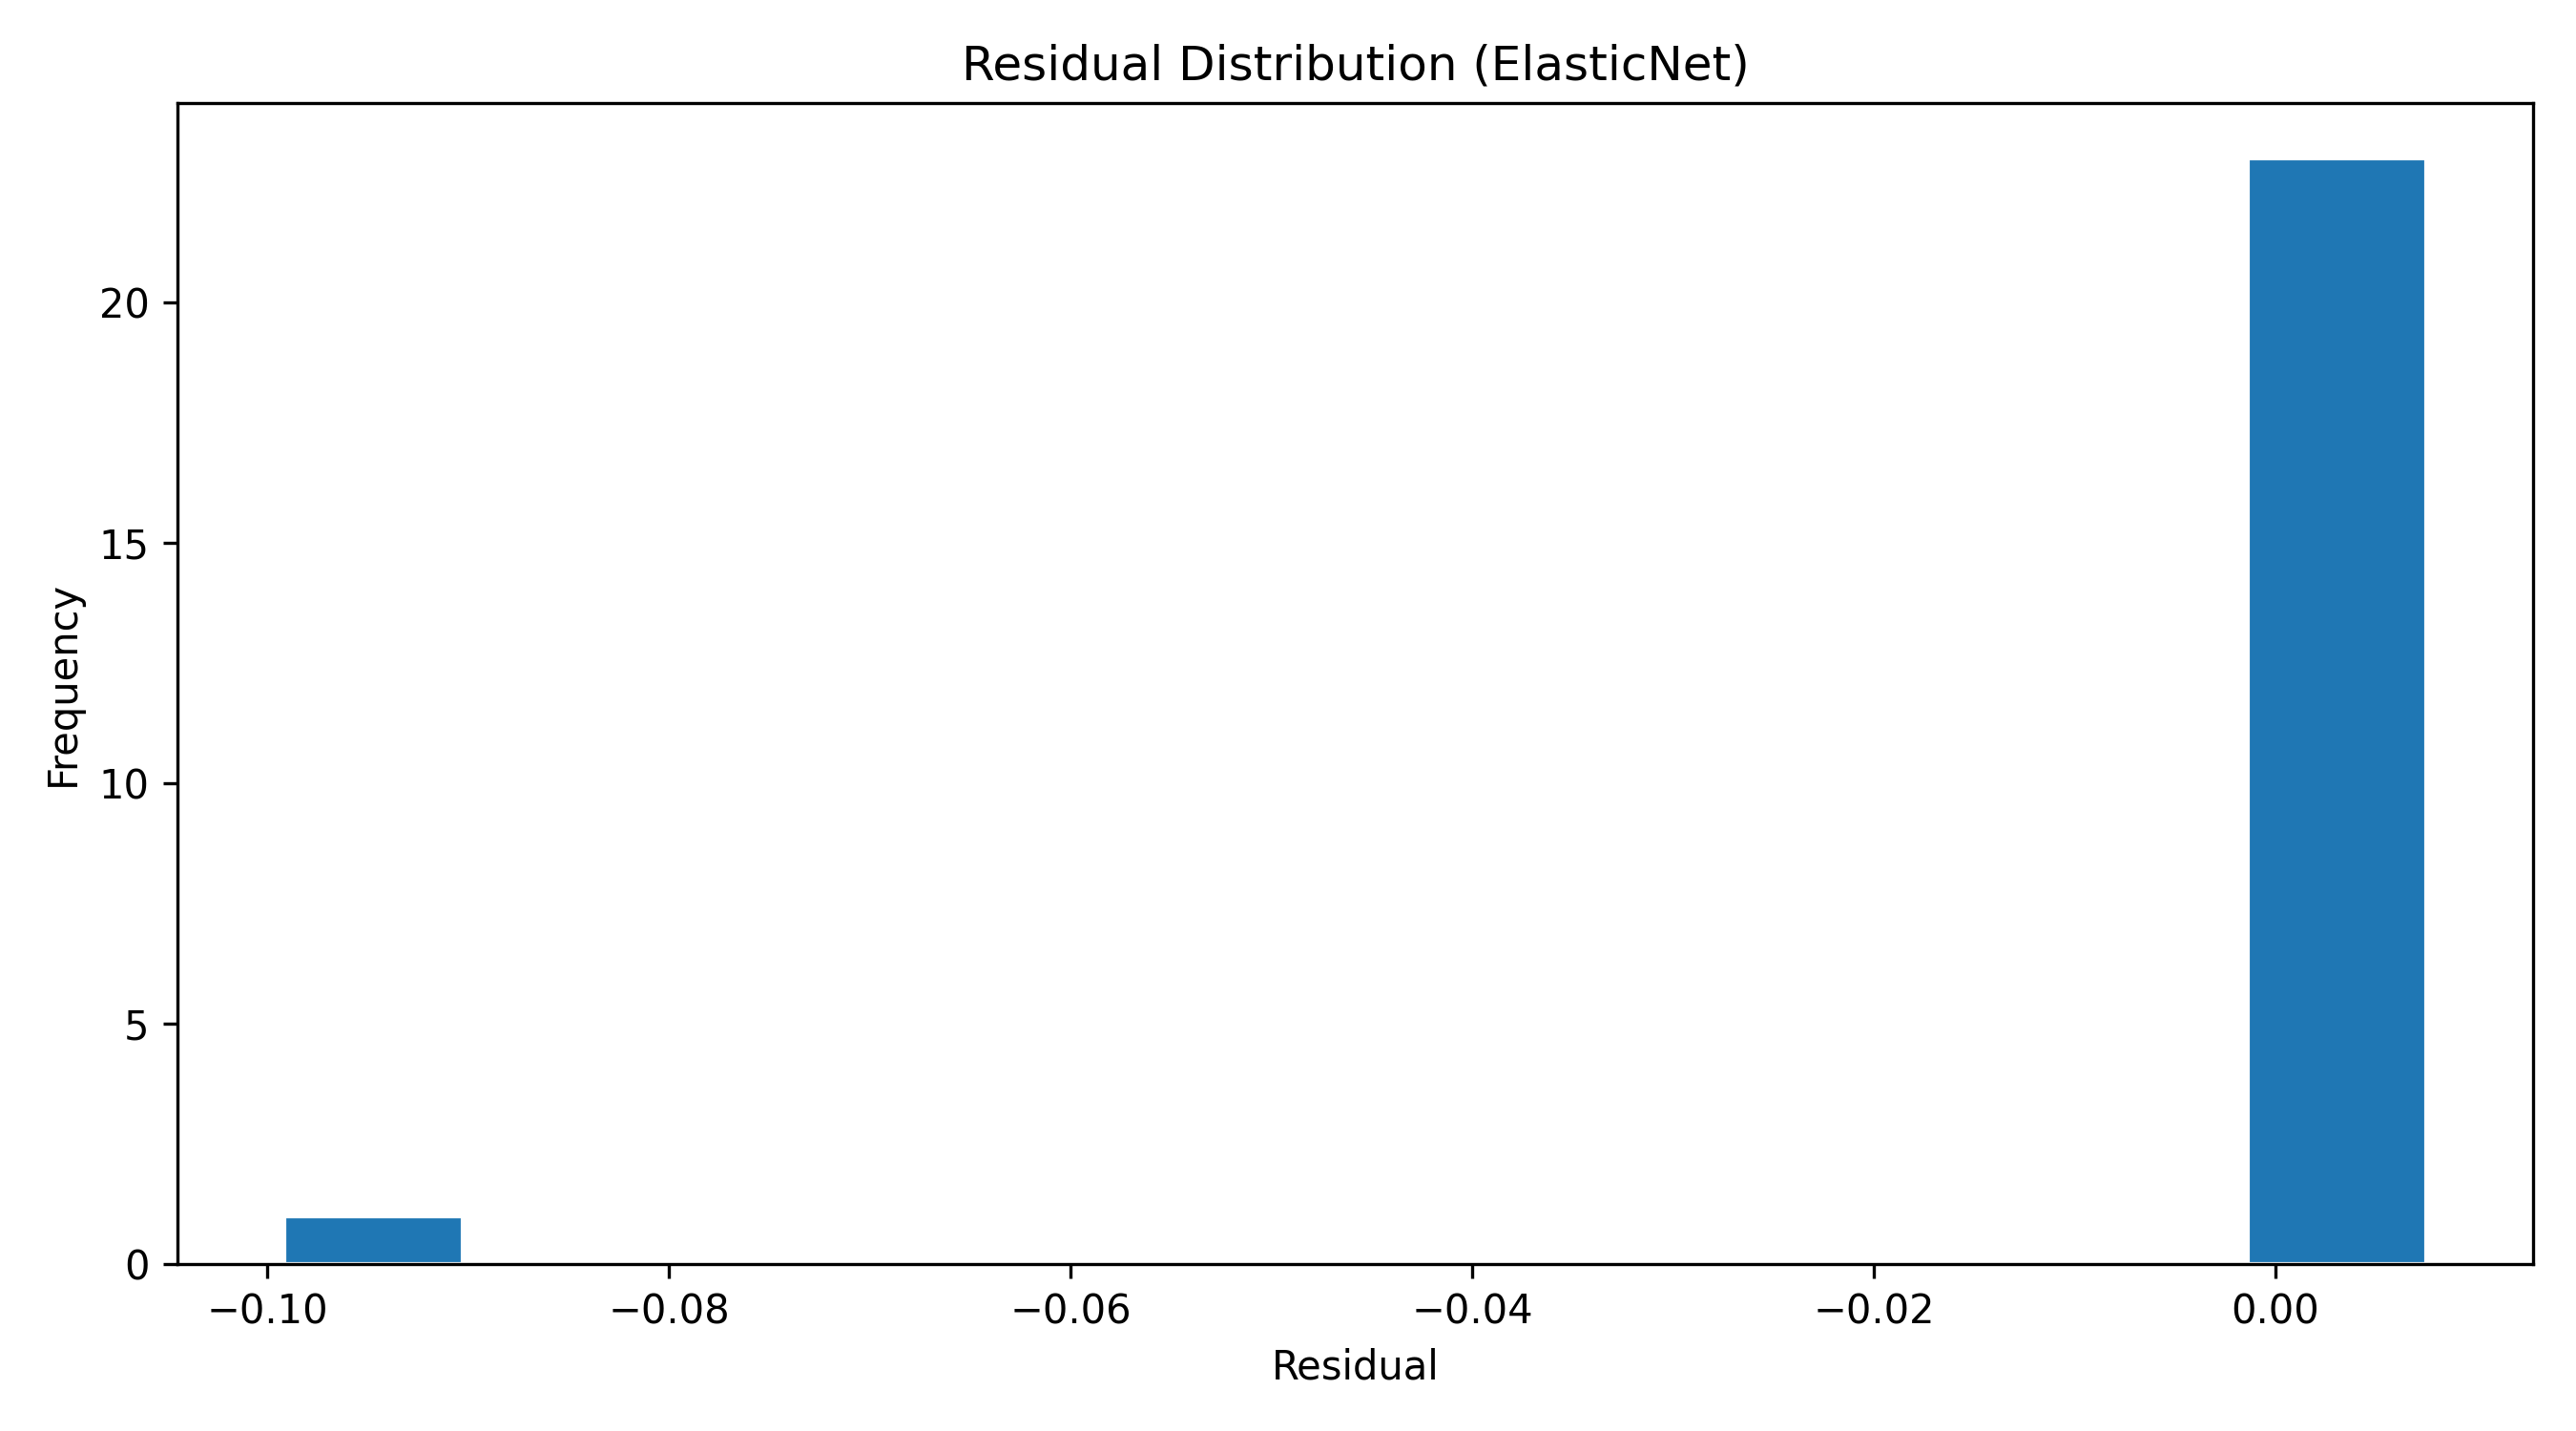
\includegraphics[width=0.7\textwidth]{figures/residual_distribution.png}
    \caption{Residual Distribution}
\end{figure}

\begin{figure}[h!]
    \centering
    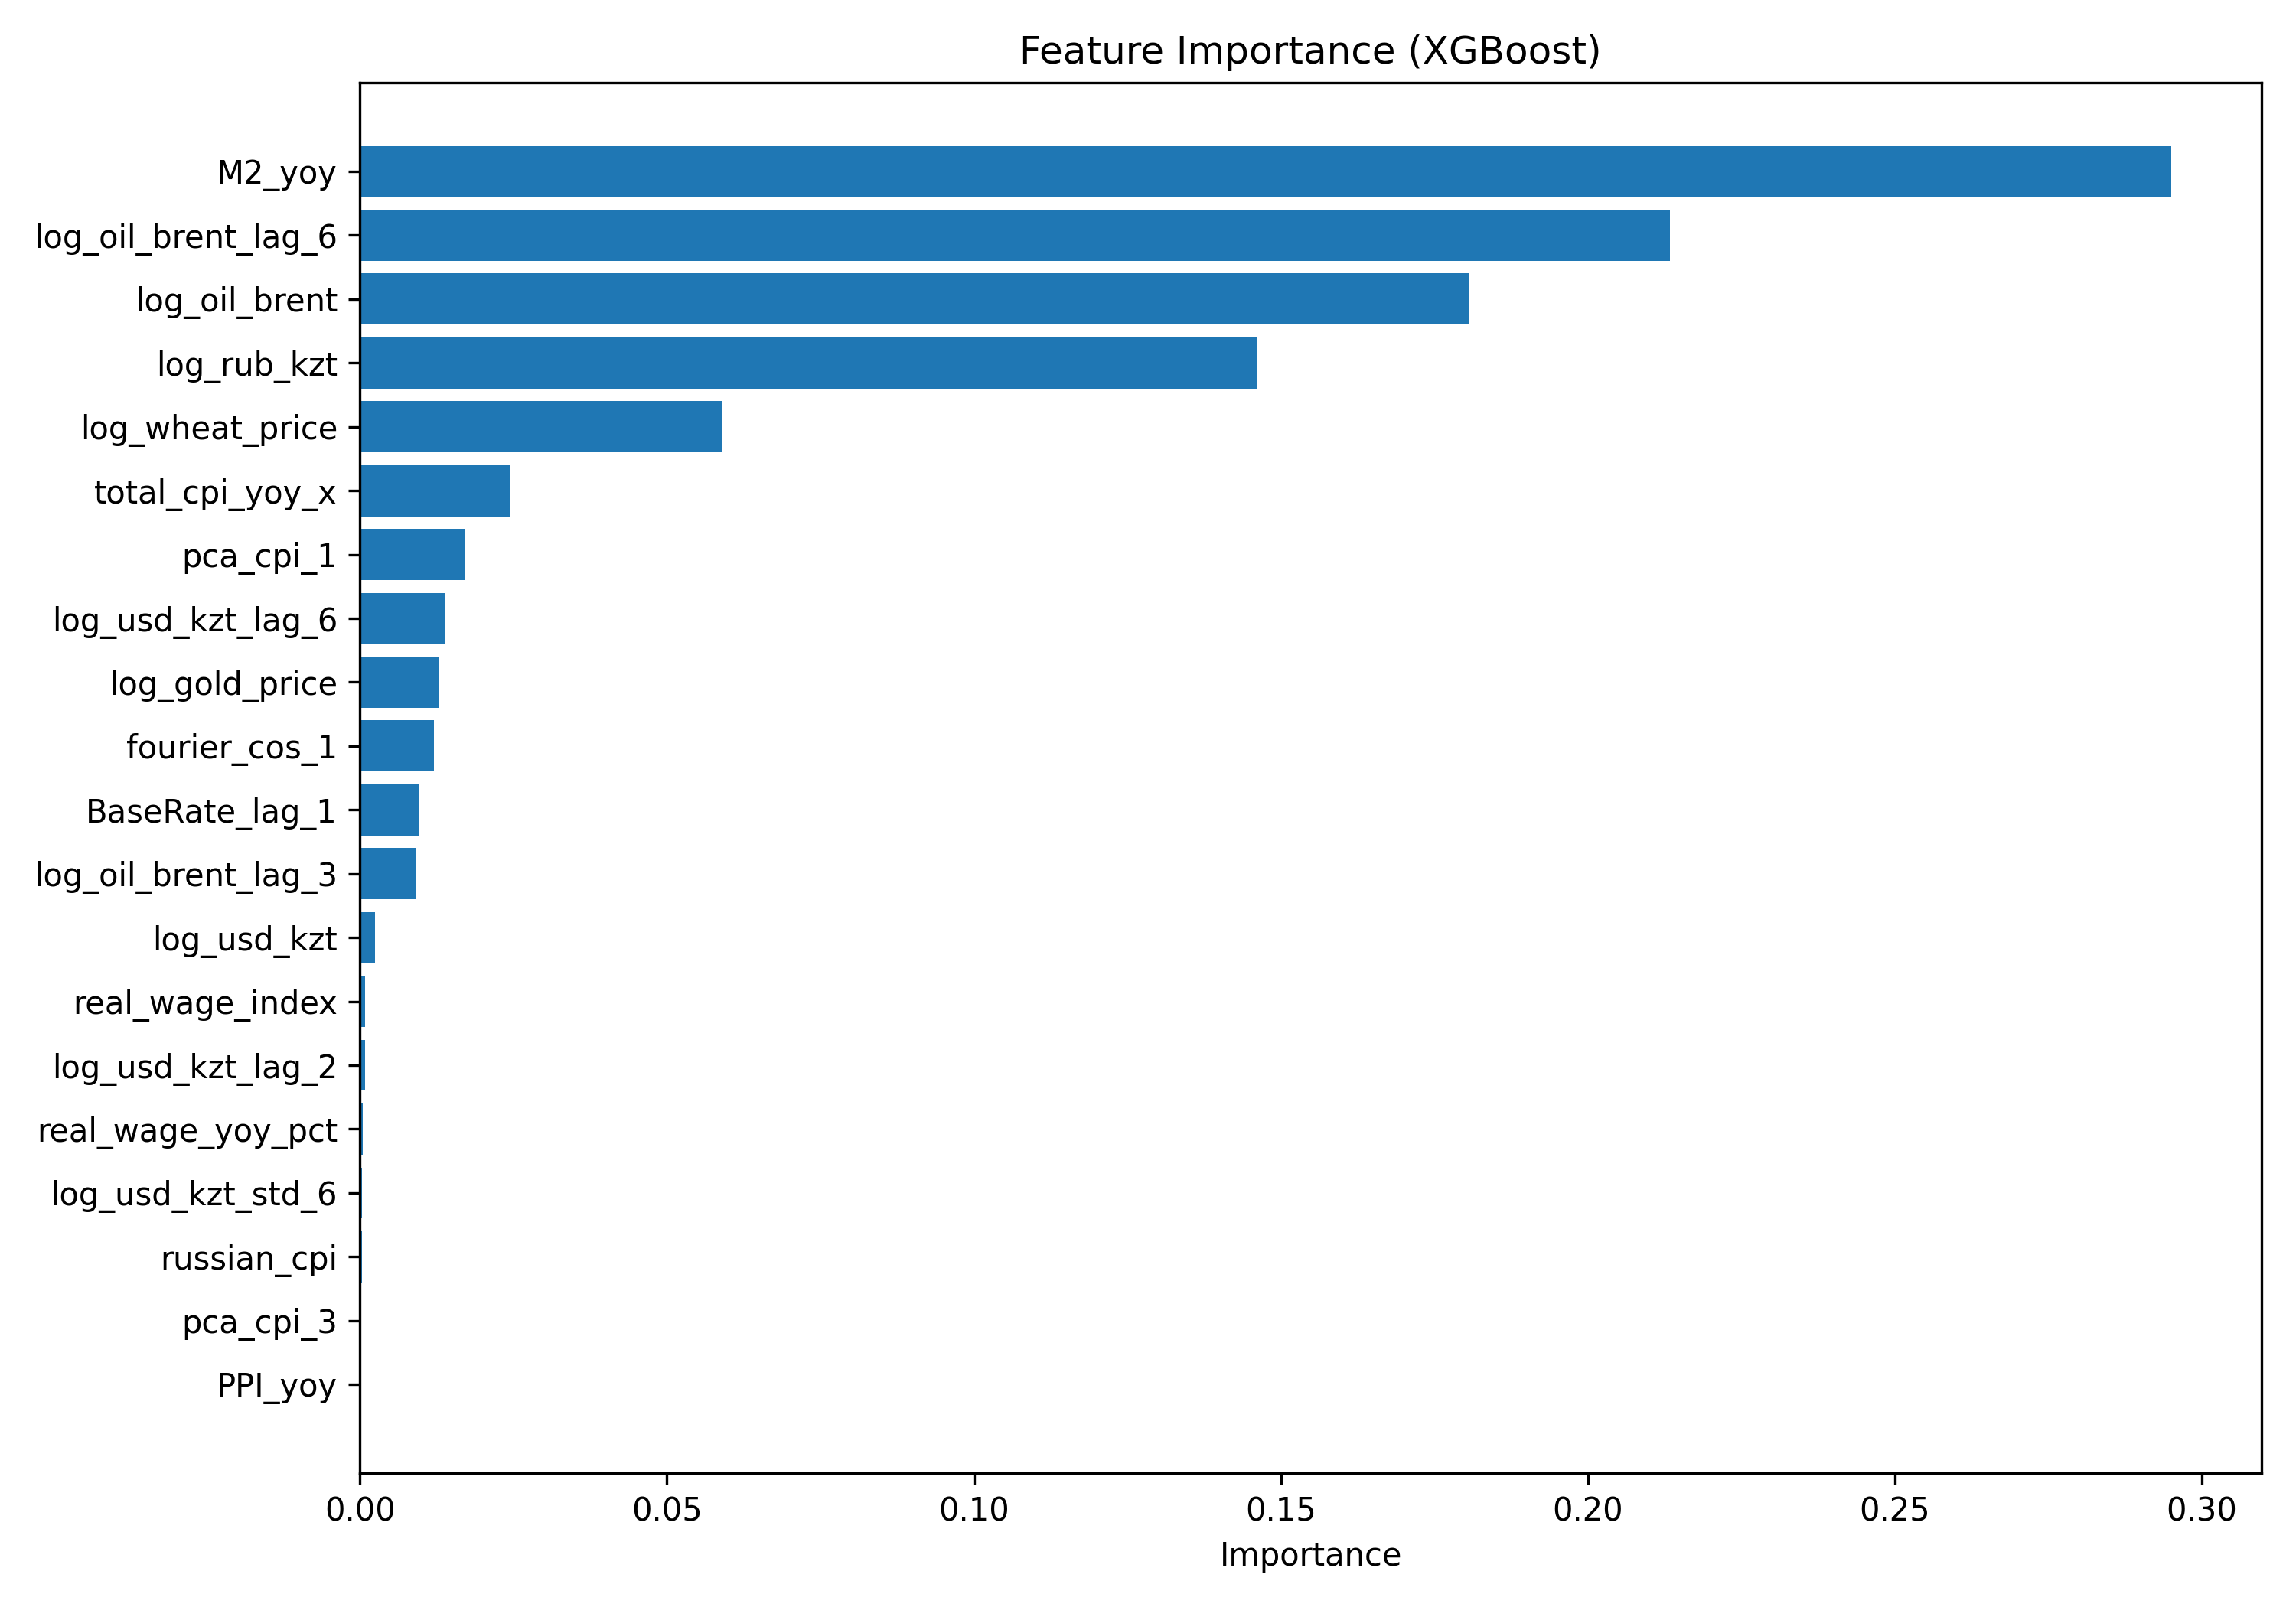
\includegraphics[width=0.8\textwidth]{figures/feature_importance.png}
    \caption{Feature Importance}
\end{figure}

\section{Conclusion}
[Summarize main findings, limitations, and suggested extensions.]

\end{document}
